\section{REST}

REST ou Representational State Transfer é um estilo de arquitetura usada para a comunicação de sistemas distribuídos através do protocolo HTTP. Foi introduzido por Roy Fielding em 2000 com o objetivo de oferecer às aplicações web um modelo de interface de acesso baseada em recursos. Além disso, descreve 6 tipos de restrições que serviços deveriam aplicar para ganho de performance, escalabilidade, simplicidade, modificabilidade, visibilidade, portabilidade e confiabilidade.

Vale lembrar que, por ter causado grande repercussão após sua publicação. O termo REST, segundo Richardson, acabou sofrendo diversas interpretações durante o tempo e, sua descrição representada de formas não originalmente propostas por Fielding. Alguns descrevem que serviços que violam essas restrições não podem ser considerados RESTful. Para Wildermuth, apesar de reconhecer as vantagens de cada restrição, serviços web devem usá-los de forma pragmática. \cite{RichardsonEtAl2013} \cite{Wildermuth2015}

Ao ser introduzido no mercado de API's, REST acabou se adaptando bem por ter se mostrado uma solução de fácil acesso em clientes web, mobile apps e IoTs\footnote{
  Internet of Things
}. Segundo Pautasso, a eliminação da complexidade existente em Web Services antes de sua publicação em 2000 fez com que REST fosse considerado um dos principais responsáveis pela popularização de arquiteturas orientada a serviços. \cite{PautassoEtAl2008}

\begin{figure}[H]
  \centering    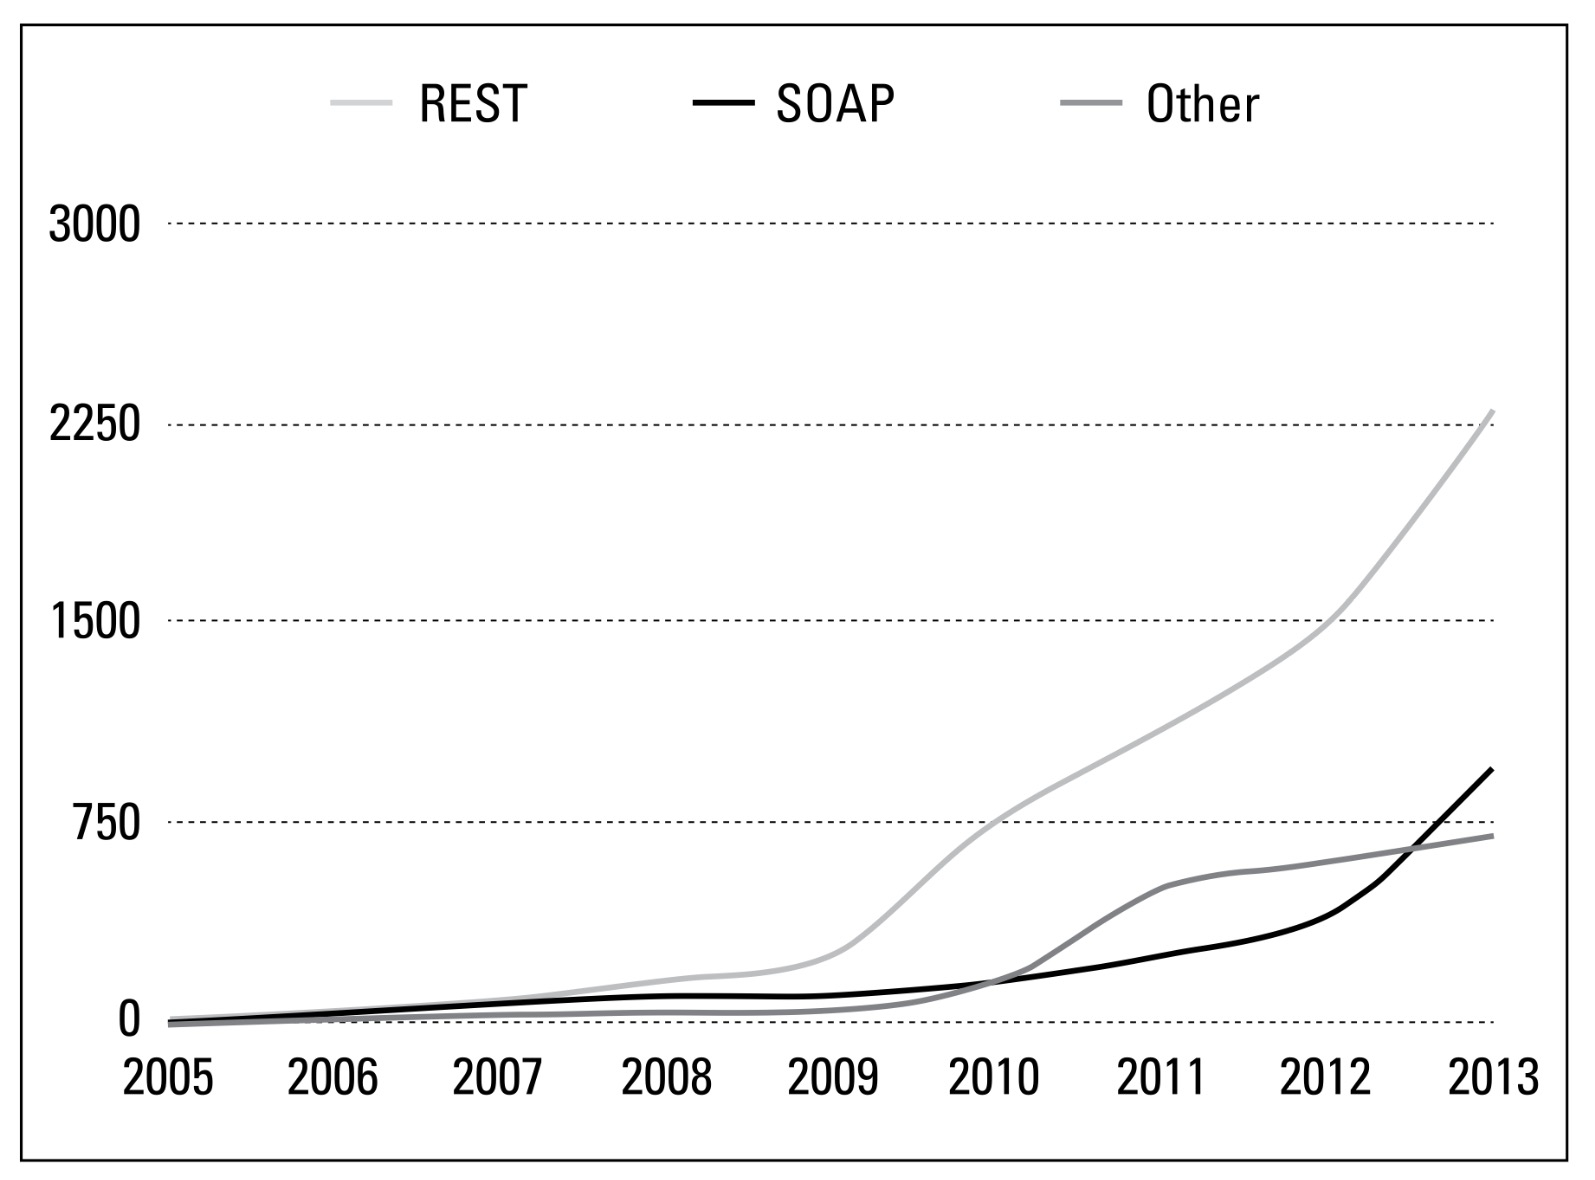
\includegraphics[width=0.9\textwidth,height=\textheight,keepaspectratio]{figuras/api-styles.jpg}
  \caption{Distribuição de estilos e protocolos para API's}
\end{figure}

A seguir será feita uma abordagem sobre os 6 tipos de restrições propostas por Fielding, o que é o termo RESTful, além de entrar em detalhe sobre as atuais soluções para descrição de API's.

\subsection[Restrições de Arquitetura]{Restrições de Arquitetura}

Esta seção fornece uma visão geral sobre as restrições propostas por Fielding para a implementação em arquiteturas web, além de ser examinado o impacto de cada restrição nesses sistemas distribuídos. \\

\textbf{Cliente-Servidor} \\

Nesta primeira restrição, não existe conexão entre cliente e servidor, mas sim a espera do servidor por pedidos de clientes através de chamada e resposta. O cliente (consumidor do serviço) não se preocupa com tarefas de comunicação de banco de dados, gerenciamento de cache, entre outros. Assim como o servidor (prestador de serviços) não está preocupado com as tarefas do cliente como interface ou experiência do usuário por exemplo. Permitindo a evolução independente dos dois ambientes, \textit{desde que sua interface de comunicação não seja alterada}. \cite{Fielding2000} \\

\textbf{Sem Estado} \\

Esta restrição ajuda na viabilidade, confiabilidade e escalabilidade de sistemas distribuídos, pois garantem que chamadas à API não estejam vinculadas a um determinado servidor. Como HTTP é um protocolo sem conexão, cada requisição deve conter todas as informações necessárias para que um servidor entenda o que um cliente está executando. Para Wildermuth, no entanto, dependendo da diversidade no número de clientes, ao manter um servidor sem estado, perder-se o controle no tamanho da estrutura de resposta necessária para atender a demanda de todos os clientes. \cite{Wildermuth2015} \\

\textbf{Interface Uniforme} \\

Em essência, Fielding propõe que aplicações façam o uso de verbos HTTP (POST, GET, PUT, DELETE) e identificadores uniforme de recursos (URI) para mapear operações em ambientes distribuidos e minimizar o acoplamento entre cliente-servidor. Essas regras de acesso são: \cite{Fielding2000}

\begin{itemize}[noitemsep]
\item Identificação de Recursos: Cada recurso deve ser disponibilizado através de uma URI específica e coesa. (Exemplo: GET /customers/1)
\item Manipulação de Recursos através de Representações: Um recurso pode ser representado em diferentes formatos para diferentes clientes. (Exemplo: HTML, XML, JSON)
\item Resposta Auto-explicativa: Metadados devem ser adicionados na requisição e resposta de um recurso para descrever seu estado atual ou desejado. (Exemplo: código de resposta HTTP, Host, Content-Type)
\item HATEAOS\footnote{
  Hypermedia as the Engine of Application State.
} - Caso um recurso possua relacionamentos, ao ser representado, estes devem estar especificados em forma de hiperlinks para facilitar a navegação de dados por clientes.
\end{itemize}

\textbf{Separação em Camadas} \\

Um dos princípios desta restrição está em evitar que clientes façam diretamente requisição para o servidor sem antes passar por um intermediário, como por exemplo um load balancer\footnote{
  Técnica para distribuir a carga de trabalho uniformemente entre dois ou mais computadores
}. Assegurando que clientes apenas se preocupem com a comunicação, deixando para que intermediários lidem com a distribuição de requisições. \cite{Fielding2000}

\begin{figure}[H]
  \centering  	   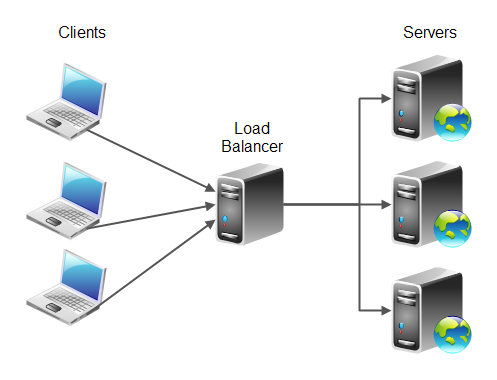
\includegraphics[width=0.7\textwidth,height=\textheight,keepaspectratio]{figuras/load-balancer.png}
  \caption{Exemplo de Load Balancer}
\end{figure}

\textbf{Código sob Demanda} \\

Apesar de ser a única restrição opcional do estilo, ela permite que servidores disponibilizem código em forma de script para que seja executado no cliente. Dessa forma, extendendo a lógica de serviço do servidor para seus clientes. \cite{Fielding2000} \\

\textbf{Cache} \\

Para aumentar desempenho de um serviço. Quando um recurso é acessado por mais de um cliente, se não houve mudança neste é recomendado que estas respostas sejam armazenadas em cache, evitando o processamento desnecessário. Isso significa que servidores, quando possível, devem implementar regras de cache para beneficio de ambos os ambientes. \cite{Fielding2000}

\subsection[RESTful]{RESTful}

Segundo Richardson, para que uma API de estilo REST seja consideirado RESTful, esta precisa seguir estritamente as regras exigidas anteriormente. Além disso, Richardson propõem uma escala de 4 níveis para avaliar a coesão e maturidade dessas APIs. \cite{RichardsonEtAl2013}

\begin{itemize}[noitemsep]
\item \textbf{Nível 0}: É a falta de qualquer regra; diz respeito ao uso de HTTP para operações de endereços no servidor. Normalmente, usa apenas um endpoint (URI) e um verbo HTTP.
\item \textbf{Nível 1}: Aplicação de recursos. A API é dividida em diferentes endpoints que indicam um ou mais recursos.
\item \textbf{Nível 2}: Implementação de verbos HTTP para diferentes tipos de operações. Onde uma mesma URI pode aceitar mais de um verbo para excução de diferentes procedimentos.
\item \textbf{Nível 3}: O conceito de HATEOS é aplicado para disponibilizar informações necessárias para interação e navegação da API.
\end{itemize}

\begin{figure}[H]
  \centering
  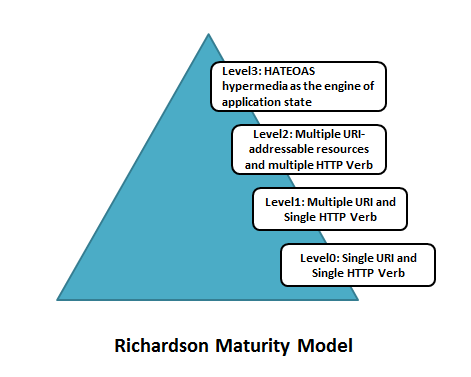
\includegraphics[width=0.8\textwidth,height=\textheight,keepaspectratio]{figuras/richardson-maturity-model.png}
  \caption{Modelo de Maturidade descrito por Richardson}
\end{figure}

\subsection[Descrição de API]{Descrição de API}

Atualmente, o processo de descrição de API's tem-se tornado um dos principais fatores de sucesso na aceitação de serviços por desenvolvedores. No entanto, diferente do processo de implementação, a prática de descrição de API's REST ainda continua sendo feita em sua maior parte manualmente através de linguagem natural. Isso porque REST não apresenta uma forma de documentação externa para descrição de pontos de acesso. \cite{LuckyEtAl2016}
 
Ao invés, Fielding propõe a descrição dinâmica de API's através do uso de hiperlinks na representação de recursos para navegação de dados (HATEOS). Contudo, para Knupp, a solução proposta por Fielding é questionável, pois na sua visão dificulta a legibilidade da interface de acesso, não prevê documentação, cria complexidade de implementação e aumenta de forma significativa o tamanho de resposta. \cite{Knupp2016}

Em busca de oferecer uma solução simples e completa para descrição de API's REST, foram introduzidas nos últimos anos diversas soluções por empresas e comunidades de desenvolvimento. A seguir, são descritas três das linguagens e formatos que maior ganharam popularidade devido a sua facilidade de uso e legibilidade por humanos e máquinas. \cite{Sandoval2015}
 
\begin{description}[leftmargin=8em,style=nextline]
  \item[\textbf{OpenAPI}] \textbf{Pros}: Amplamente adotada, ampla comunidade, suporte à diversas linguagens. \\ \textbf{Cons}: Carece de especificações avançadas de metadados.
  \item[\textbf{RAML}] \textbf{Pros}: Suporte à especificação avançada de metadados, adoção significativa, formato legível, suporte da indústria. \\ \textbf{Cons}: Falta de ferramentas de auxílio, não comprovada à longo prazo.
  \item[\textbf{API Blueprint}] \textbf{Pros}: Fácil de entender e simples de escrever \\ \textbf{Cons}: Pouca adoção, carece de especificações avançadas de metadados, difícil de executar.
\end{description}

Enquanto HATEOS continuar tendo baixa adoção e não houver a padronização de um formato externo para descrição de API's, novas tecnologias estão propensas a surgir pela comunidade para melhor ocupar esta posição. Uma delas, não mencionada anteriormente é o JSON Hyper-Schema que, recentemente através de Lynn e Leach, mostrou ser um método simples e completo para modelagem de API's REST. Uma vez que possui suporte à descrição de representação de entrada e saída, relacionamentos, HATEOS, URIs e verbos HTTP  \cite{LynnEtAl2016} \cite{Leach2014}.

